\documentclass[11pt, a4paper]{article}
\usepackage[utf8]{inputenc}
\usepackage{t1enc}
\usepackage[magyar]{babel}
\usepackage{lmodern}
\usepackage{url}
\usepackage{graphics}
\usepackage{listings}
\usepackage[a4paper, total={5.3in, 8in}]{geometry}

\sloppy

\begin{document}
\title{Szoftver architektúrák \\ Szótanulást segítő alkalmazás \\ \large{Rendszerterv}}
    \author{Graics Bence \and Verbőczy Kristóf}

    \maketitle
    
    \tableofcontents
    \newpage
    
    \section{Bevezetés}
    \label{sec:bevezetes}
    Jelen dokumentum a Szoftver architektúrák nevű tárgyra kidolgozott házi feladat rendszertervet mutatja be. A házi feladat során a cél egy szótanulást segítő alkalmazás megtervezése és implementálása volt. Az alkalmazással kapcsolatos követelmény specifikációt a \textit{https://www.aut.bme.hu/} tanszéki oldal \textit{Eredmények} oldalára töltöttük fel.
    
    A dokumentum a következők szerint épül fel. \Aref{sec:architektúra}.~fejezet bemutatja az alkalmazás architektúráját, a terveket, illetve pár érdekes megvalósítási részletet. \Aref{sec:telepítés}.~fejezet megmutatja, hogyan lehet telepíteni és elindítani az alkalmazást. Végül \aref{sec:összefoglalás}.~fejezet összefoglalja a munkánkat és továbbfejlesztési lehetőségeket mutat be.
    
    \section{Architektúra}
    \label{sec:architektúra}
    Jelen fejezet bemutatja az elkészített szótanuló alkalmazás architektúráját, azaz hogy \textit{1)} a rendszer milyen komponensekből épül fel, \textit{2)} az egyes komponenseknek milyen lényeges elemei vannak, \textit{3)} a komponensek hogyan kapcsolódnak egymáshoz.
    
    Az általunk tervezett rendszer egy adatközpontú alkalmazás, amely \emph{kliens-szerver} architektúrát követ. A szerver tárolja a szükséges adatokat, például a felhasználók adatait és az egyes leckékhez tartozó adatokat (szavakat és képeket). A kliens feladata, hogy a felhasználó kérésére fogyasztható formában tárja a felhasználó elé ezen adatokat, és kezelje az esetleges interakciókat. Az adatok (az objektum-orientáltság szabályai szerint) objektumokban (DTO) kerülnek továbbításra és feldolgozásra. A szerver és a kliens kommunikációját jól meghatározott interfészek teszik lehetővé.
    
    \subsection{Objektumok}
    A kliens és a szerver az adatokat objektumokban tárolják, és ezek kerülnek sorosításra, illetve visszasorosításra, amikor kommunikáció történik a két fél között. Az alkalmazás a által támogatott objektumokat \aref{fig:objects-uml}.~ábra mutatja be.
    
    \begin{figure}[htbp]
    	\center
    	\resizebox{140mm}{!}{
    		\includegraphics{figures/objects-uml.pdf}
    	}
    	\caption{Osztálydiagram a támogatott objektumokról.}
    	\label{fig:objects-uml}
    \end{figure}
    
    \paragraph{ExerciseType} Egy enumeráció, amely a lehetséges feladat típusokat (mondat lefordítása, helyes szó kiválasztása, kép leírása) definiálja.
    
    \paragraph{KnowledgeLevel} Egy enumeráció, amely különböző feladat nehézségi szinteket, illetve felhasználói tudásszinteket definiál: kezdő, haladó, szakértő.
    
    \paragraph{Exercise} Egy osztály, amely egy ``mondat lefordítása'' feladatot szimbolizál. Tartalmaz egy angol és egy magyar sztringet mint szópárt.
    
    \paragraph{ExerciseWithImage} Egy osztály, amely egy ``kép leírása'' feladatot szimbolizál. Az Exercise osztályból származik le. Az ősének a mezői mellett tartalmaz egy képet is, amelyet a felhasználónak le kell írnia.
    
    \paragraph{FourWordsExercise} Egy osztály, amely egy ``helyes szó kiválasztása'' feladatot szimbolizál. Az Exercise osztályból származik le. Az ősének a mezői mellett tartalmaz sztring listát, amely a lehetséges rossz válaszokat tartalmazza.
    
    \paragraph{SentenceExercises} Egy csomagolóosztály, ``mondat lefordítása'' feladatokat tartalmaz.
    
    \paragraph{ImageExercises} Egy csomagolóosztály, ``kép leírása'' feladatokat tartalmaz.
    
    \paragraph{FourWordsExercises} Egy csomagolóosztály, ``helyes szó kiválasztása'' feladatokat tartalmaz.
    
    \textbf{Megjelenés a kódban:} \textit{language.learning.exercise} package-ben található enumerációk és osztályok.
    
    \subsection{Interfészek}
    \label{sec:interfészek}
    
    A kliens és a szerver közötti kommunikációt jól definiált interfészek teszik lehetővé. Az interfészeken és a deklarált metódusaikon különböző annotációk találhatók, amelyek a hálózati REST kommunikációhoz szükségesek. Ezekkel lehet definiálni az elérési útvonalat (path), a REST metódust (POST, PUT, DELETE, GET), illetve a hálózaton közlekedő adatnak a formátumát (XML vagy JSON).
    
    A funkcionalitást három interfész definiálja: ILearning, IExerciseManager és IUserManager. Az interfészek a következőképpen épülnek fel.
    
    \paragraph{ILearning} Ez az interfész a tanulással és a felhasználók tanulással szerzett pontjainak menedzselésével kapcsolatos funkcionalitást írja le. Metódusai:
    \begin{itemize}
    	\item SentenceExercises getSentenceExercises(String userLevel, boolean equals, int count): adott számú (count) ``mondat lefordítása'' feladat visszaadását teszi lehetővé a felhasználó szintjének megfelelően (userLevel), illetve attól függően, hogy csak a felhasználó szintjéről, vagy alacsonyabb szintű feladatokból is lehet a feladatokat választani (equals).
    	
    	\item FourWordsExercises getWordExercises(String userLevel, boolean equals, int count): adott számú ``helyes szó kiválasztása'' feladat visszaadását teszi lehetővé.
    	
    	\item ImageExercises getImageExercises(String userLevel, boolean equals, int count): adott számú ``kép leírása'' feladat visszaadását teszi lehetővé.
    	
    	\item void updateUserScore(int score, User user): egy felhasználó tapasztalati pontjainak a számának a változtatását teszi lehetővé.
    	
    	\item void updateUserLevel(String userLevel, User user): egy tudásszintjének a változtatását teszi lehetővé.
    \end{itemize}
    \paragraph{IExerciseManagement} Ez az interfész a feladatok menedzsmentjével kapcsolatos funkcionalitást írja le. Metódusai:
    \begin{itemize}
    	\item void addExercise(String username, Exercise exercise): egy egyszerű feladat (angol-magyar szópár vagy mondatpár) regisztrálását teszi lehetővé.
    	
    	\item void addExercise(String username, ExerciseWithImage exercise): egy  ``kép leírása'' feladat regisztrálását teszi lehetővé.
    	
    	\item void deleteExercise(String username, Exercise exercise): egy feladat törlését teszi lehetővé.
    	
    	\item SentenceExercises listExercises(): lehetővé teszi az összes feladat (angol-magyar szópár) lekérését.
    \end{itemize}
    
    \paragraph{IUserManagement} Ez az interfész a felhasználók menedzsmentjével kapcsolatos funkcionalitást írja le (adminisztrátorok feladatai). Metódusai:
    \begin{itemize}
   	\item User logIn(String username): Lehetővé teszi egy felhasználó lekérését egy felhasználónév alapján.
   	
   	\item boolean addUser(User user): Egy felhasználó regisztrálását teszi lehetővé.
   	
   	\item void deleteExercise(String username, Exercise exercise): Lehetővé teszi egy feladat törlését.
   	
   	\item boolean deleteUser(String username): Egy felhasználó törlését teszi lehetővé.
   \end{itemize} 
   
    
    \textbf{Megjelenés a kódban:} \textit{language.learning.server} package-ben található interfészek.
    
    \subsection{A szerver}
    A szerver rétegelt architektúrája négy fő részre bontható. Ezek az alábbiak:
    \begin{itemize}
    	\item szolgáltatás hozzáférési réteg (Rest API),
    	\item üzleti logika réteg,
    	\item adatelérési réteg,
    	\item adatbázis réteg.
    \end{itemize}
    A közöttük lévő kapcsolatot mutatja be \aref{fig:server_arch}. ábra.
    
    \begin{figure}[htbp]
    	\center
    	\resizebox{140mm}{!}{
    		\includegraphics{figures/server_architecture.pdf}
    	}
    	\caption{A szerver architekturális felépítése.}
    	\label{fig:server_arch}
    \end{figure}
    
    \subsubsection{Szolgáltatás hozzáférési réteg}
    Az a réteg egy REST API-nak felel meg, amelyen keresztül http kérésekkel és erre adott http válaszokkal lehet igénybe venni a szerver szolgáltatását (lásd \ref{sec:interfészek}.~fejezet).
    
    \textbf{Megjelenés a kódban:} \textit{language.learning.server} package-ben található interfészek: 
    \begin{itemize}
    	\item ILearning
    	\item IExerciseManager
    	\item IUserManager
    \end{itemize}
    
    A fejlesztés során lehetőség volt a program kliens nélküli tesztelésére, hiszen elég http kéréseket küldeni neki. Erre a \textit{Postman}\footnote{https://www.getpostman.com/} nevezetű programot használtuk.
    
    \subsubsection{Üzleti logika réteg}
    Ez a réteg a szolgáltatás interfészek konkrét megvalósításaiból áll. Feladata adatelérési réteg megfelelő metódusainak meghívása, és az eredmény az interfészben definiált formára hozása. Erre jó példa, hogy véletlenszerűen kell visszaadnia a szervernek N darab feladatot, ahol N-t a kliens kérése határozza meg. Ez a feladat tipikusan üzleti logika hatáskörébe tartozik.
    
    \textbf{Megjelenés a kódban:} \textit{language.learning.server} package-ben található osztályok: 
    \begin{itemize}
    	\item Learning
    	\item ExerciseManager
    	\item UserManager
    \end{itemize}
    
    \subsubsection{Adatelérési réteg}
    Feladata az adatbázishoz való hozzáférés, melynek során biztosítja a szükséges \textit{lekérdezéseket, beszúrásokat, módosításokat, törléseket}. Ezen a szinten történik a védekezés az SQL injection ellen, a \textit{java.sql.PreparedStatement} interfész segítségével.
    
    \textbf{Megjelenés a kódban:} \textit{language.learning.database} package-ben IDatabase interfész, és ennek a megvalósítása a Database osztály.
    
    Az adatbázis elérésére az Oracle JDBC 7-es verziójú drivere került felhasználásra, ezt a kódban a Database osztályban meg is kell adni.
    
    \subsubsection{Adatbázis réteg}
    Feladata az adatok perzisztens tárolása. A használt adatbázis az Oracle Database 11g Express Edition\footnote{http://www.oracle.com/technetwork/database/database-technologies/express-edition/overview/index.html}. Azért erre esett a választás, mert ingyenes, és mivel korábbi ismereteink és tapasztalataink az Oracle adatbázisokhoz voltak köthetők, ezért mindenféleképpen Oracle terméket szerettünk volna használni. Bár vannak újabb verziók is, a 11g verzió stabilnak és elterjedtnek mondható, ezért döntöttünk emellett.
    
   \textbf{ Megjelenés a kódban:} nem írtunk hozzá komponenst, viszont a függőségek között megjelenik az ojdbc7.jar, ami szintén ingyenesen letölthető az Oracle honlapjáról\footnote{http://www.oracle.com/technetwork/apps-tech/jdbc-112010-090769.html}. Érdekesség, hogy a projektünk Maven projekt, így a pom.xml-be megadott függőségek automatikusan letöltődnek, viszont az Oracle nem teszi ki publikus repository-ba az ojdbc driver-t, ezért manuálisan kell letölteni és beállítani a függőségeket.
    
    \subsection{Adatbázis terv}
    Ezen fejezetben bemutatásra kerülnek az adatbázisban elmentett \emph{entitások}. Az adatbázis egyed-kapcsolat diagramja látható \aref{fig:er_diag}. ábrán.
    
    \begin{figure}[htbp]
    	\center
    	\resizebox{140mm}{!}{
    		\includegraphics{figures/er.png}
    	}
    	\caption{A szerver architekturális felépítése.}
    	\label{fig:er_diag}
    \end{figure}
    
    \subsubsection{Word Exercise}
    Ez az entitás a szó feladatokhoz szükséges adatok tárolására alkalmas. Egy angol-magyar szópárt tárol, de az entitás könnyen kibővíthető lehetne további, más nyelvű szavakkal. Továbbá tárolja, hogy milyen nehézségű a feladat, és azt is, hogy melyik felhasználó hozta létre.
    
    Az id értékének generálására a \textit{WORDEXERCISE\_SEQ} szekvencia szolgál.
    
    \begin{table}[!h]
    	\centering
    	\begin{tabular} {|c|c|c|}
    		\hline
    		Név & Adatbázis típus & Java típus \\
    		\hline
    		id & number \textbf{(PK)} & nem jelenik meg ez a mező \\
    		english & nvarchar2(30) & String \\
    		hungarian & nvarchar2(30) & String \\
    		userid & number \textbf{(FK)} & int \\
    		knowledgelevelID & number \textbf{(FK)} & int \\
    		\hline
    	\end{tabular}
    \end{table}
    
    \subsubsection{Sentence Exercise}
    Nagyon hasonlít a \textit{Word Exercise}-ra, de ez alkalmas hosszabb karakterlánc párok eltárolására is, tehát nem csak szavakat, hanem hosszabb mondatokat is tudunk tárolni benne. Elképzelhető, hogy össze lehetne vonni a \textit{Word Exercise} és \textit{Sentence Exercise} táblákat, de akkor az új entitásban szükség lenne további attribútumok bevezetésére (pl.:~feladat típus), továbbá ez a struktúra egyértelműen tükrözi, hogy miképp válnak külön a feladattípusok.
    
    Az id értékének generálására a \textit{SENTENCEEXERCISE\_SEQ} szekvencia szolgál.
    
    \begin{table}[!h]
    	\centering
    	\begin{tabular} {|c|c|c|}
    		\hline
    		Név & Adatbázis típus & Java típus \\
    		\hline
    		id & number \textbf{(PK)} & nem jelenik meg ez a mező \\
    		english & nvarchar2(200) & String \\
    		hungarian & nvarchar2(200) & String \\
    		userid & number \textbf{(FK)} & int \\
    		knowledgelevelID & number \textbf{(FK)} & int \\
    		\hline
    	\end{tabular}
    \end{table}
    
    \subsubsection{Image Exercise}
    Annyiban különbözik a \textit{Word Exercise}-tól, hogy képes képek tárolására. Az id értékének generálására az \textit{IMAGEEXERCISE\_SEQ} szekvencia szolgál.
    
    \begin{table}[!h]
    	\centering
    	\begin{tabular} {|c|c|c|}
    		\hline
    		Név & Adatbázis típus & Java típus \\
    		\hline
    		id & number \textbf{(PK)} & nem jelenik meg ez a mező \\
    		english & nvarchar2(30) & String \\
    		hungarian & nvarchar2(30) & String \\
    		userid & number \textbf{(FK)} & int \\
    		knowledgelevelID & number \textbf{(FK)} & int \\
    		image & BLOB & byte[] \\
    		\hline
    	\end{tabular}
    \end{table}
    
    \subsubsection{Application User}
    A felhasználó adatait tartalmazza. Az egyértelmű felhasználónév, jelszón páron kívül tárolja még a pontszámát, a tudásszintjét és azt, hogy rendelkezik-e adminisztrátori jogosultsággal.
    
    Az id értékének generálására a \textit{USER\_SEQ} szekvencia szolgál.
    
    \begin{table}[!h]
    	\centering
    	\begin{tabular} {|c|c|c|}
    		\hline
    		Név & Adatbázis típus & Java típus \\
    		\hline
    		id & number \textbf{(PK)} & nem jelenik meg ez a mező \\
    		username & nvarchar2(15) & String \\
    		userpassword & nvarchar2(128) & String \\
    		userscore & number & int \\
    		knowledgelevelID & number \textbf{(FK)} & int \\
    		isadmin & number & boolean \\
    		\hline
    	\end{tabular}
    \end{table}
    
    \subsubsection{Knowledge Level}
    A különböző tudásszinteket tárolja. Mivel ezt a felhasználók nem tudják befolyásolni és kevés típus van, ezért nem szükséges szekvencia az id értékének generálására.
    
    \begin{table}[!h]
    	\centering
    	\begin{tabular} {|c|c|c|}
    		\hline
    		Név & Adatbázis típus & Java típus \\
    		\hline
    		id & number \textbf{(PK)} & nem jelenik meg ez a mező \\
    		levelname & nvarchar2(10) & enumeráció \\
    		\hline
    	\end{tabular}
    \end{table}
    
    \subsection{A kliens}
    \label{sec:kliens}
    A kliens a következő feladatokat látja el, felhasználva a szerver által nyújtott szolgáltatásokat.
    \begin{enumerate}
    	\item Megjelenít különböző adatokat. Ezen adatok tartozhatnak egy adott felhasználóhoz, pl.~név, pontszám, tudásszint, vagy tartozhat leckékhez, pl. angol szó, magyar szó, objektumot leíró kép.
    	\item Felhasználói kéréseket hajt végre az alkalmazáslogikának megfelelően. Ezek közé tartozik egy lecke megtanítása (tanítási folyamat végrehajtása), leckék kilistázása, leckék felvétele és törlése, felhasználók létrehozása és törlése (adminisztrátor felhasználó esetén).
    	\item A felhasználói kérések teljesítéséhez felveszi a kapcsolatot a szerverrel, hogy lekérje a szükséges adatokat, illetve perzisztálja adatok módosításának az eredményét.
    \end{enumerate}

	A kliens egy réteges felépítést követ, minden réteghez egy fent meghatározott feladat társul. A kliens felépítését \aref{fig:client-arch}.~ábra mutatja be.
	       \begin{figure}[h!]
	       	\center
	       	\resizebox{50mm}{!}{
	       		\includegraphics{figures/client-arch.pdf}
	       	}
	       	\caption{A kliens architektúrája.}
	       	\label{fig:client-arch}
	       \end{figure}
	
	Amint látható, a kliens egy tisztán rétegelt architektúrát valósít meg. A megjelenítési réteg csak az üzleti logikai réteg  nyújtotta szolgáltatásokat használja fel, az üzleti logikai réteg pedig csak a szolgáltatás hozzáférési rétegre támaszkodik. Az alkalmazásban egy réteget egy-egy osztály/fájl valósít meg. A következő szekciók részletesebben bemutatják az egyes rétegek megvalósítását.
     
     \subsubsection{Megjelenítési réteg: View fájl}
     A View fájl felelős a grafikus felhasználói felület megvalósításáért. A grafikus felület a JavaFX FXML\footnote{https://docs.oracle.com/javafx/2/get\_started/fxml\_tutorial.htm} technológia felhasználásával került definiálásra. Ennek segítségével a felületen található vezérlőket deklaratív jelleggel lehet definiálni az XML szintaktikának megfelelően: vezérlő hierarchiákat lehet létrehozni, illetve az egyes vezérlők tulajdonságait lehet definiálni (méret, szín, elrendezési algoritmus). A következő kódrészlet a bejelentkezéshez szükséges vezérlők definiálását mutatja be.
     
\begin{lstlisting}[
basicstyle=\small, %or \small or \footnotesize etc.
]
<HBox fx:id="connectionLayout" alignment="CENTER_LEFT"
	spacing="10">
<!-- Username field -->
<TextField fx:id="userNameField" maxWidth="200" maxHeight="27"
minWidth="100" minHeight="28" prefWidth="200" prefHeight="27" 
	promptText="User name" />	
<!-- Password field -->
<PasswordField fx:id="passwordField" prefWidth="200" 
	prefHeight="27" promptText="Password" />	
<Pane HBox.hgrow="ALWAYS" />
<!-- Connect button -->			
<Button fx:id="connectButton" text="Connect" prefWidth="100" 
	onAction="#connectEventHandler" />
</HBox>
\end{lstlisting}
     
     A grafikus felület egy \emph{egyablakos} megközelítést követ; az egyes funkciók különböző \emph{füleken} keresztül érhetők el. A következőkben bemutatjuk a legfontosabb képernyőket, amelyek az alkalmazás jelentősebb funkcionalitásaihoz tartoznak.
     
     A program indulása utána a következő képernyő fogad (lásd \ref{fig:connect}.~ábra).     
     \begin{figure}[h!]
	     \center
	     \resizebox{110mm}{!}{
		     \includegraphics{figures/connect.png}
	     }
	     \caption{A bejelentkező képernyő.}
	     \label{fig:connect}
     \end{figure} 
     Ekkor a felhasználónak lehetősége van bejelentkezni. Rossz felhasználónév vagy jelszó esetén az alkalmazás egy felugró ablakkal figyelmeztet (\ref{fig:login-error}.~ábra).
     \begin{figure}[h!]
     	\center
     	\resizebox{80mm}{!}{
     		\includegraphics{figures/login-error.png}
     	}
     	\caption{Rossz felhasználónév vagy jelszó esetén a hibaüzenet ablak.}
     	\label{fig:login-error}
     \end{figure}
     Bejelentkezés után a felhasználó megvizsgálhatja jelenlegi pontjait, tudás szintjét, illetve ki is jelentkezhet (\ref{fig:after-connect}.~ábra).     
     \begin{figure}[h!]
     	\center
     	\resizebox{110mm}{!}{
     		\includegraphics{figures/after-connect.png}
     	}
     	\caption{A kezdőablak bejelentkezés után.}
     	\label{fig:after-connect}
     \end{figure}
     A tanulást, azaz egy lecke megkezdését a \emph{Start Learning!} gombra kattintva kezdheti el, ahol a három különböző feladattípushoz a következő képernyők tartoznak (\ref{fig:exercise-word}., \ref{fig:exercise-sentence}. és \ref{fig:exercise-image}.~ábra).
     \begin{figure}[h!]
     	\center
     	\resizebox{110mm}{!}{
     		\includegraphics{figures/exercise-word.png}
     	}
     	\caption{Feladat: helyes szó kiválasztása.}
     	\label{fig:exercise-word}
     \end{figure}
	 \begin{figure}[h!]
	 	\center
	 	\resizebox{110mm}{!}{
	 		\includegraphics{figures/exercise-sentence.png}
	 	}
	 	\caption{Feladat: angol mondat lefordítása.}
	 	\label{fig:exercise-sentence}
	 \end{figure}
	\begin{figure}[h!]
		\center
		\resizebox{110mm}{!}{
			\includegraphics{figures/exercise-image.png}
		}
		\caption{Feladat: a kép által ábrázolt objektum megadása.}
		\label{fig:exercise-image}
	\end{figure}
     Leckék kezelését (hozzáadás, törlés, listázás) a felhasználó a \emph{Manage Exercises} fülön végezheti (\ref{fig:manage-exercises}.~ábra).
     \begin{figure}[h!]
     	\center
     	\resizebox{110mm}{!}{
     		\includegraphics{figures/manage-exercises.png}
     	}
     	\caption{A leckék kezelését segítő ablak.}
     	\label{fig:manage-exercises}
     \end{figure}
     Végül a grafikus felületen található egy adminisztrációs felület is (\emph{Manage Users}), amelyet adminisztrátor felhasználók vehetnek igénybe (\ref{fig:manage-users}.~ábra). Itt lehet felhasználókat törölni, illetve új felhasználókat hozzáadni az alkalmazáshoz.    
     \begin{figure}[h!]
     	\center
     	\resizebox{110mm}{!}{
     		\includegraphics{figures/manage-users.png}
     	}
     	\caption{A leckék kezelését segítő ablak.}
     	\label{fig:manage-users}
     \end{figure}
 
 	\textbf{Megjelenés a kódban:} \textit{src/main/resources} mappában a \textit{View.fxml} fájl.
   
     \subsubsection{Üzleti logika: Controller osztály}
     A Controller osztály felelős a felhasználói interakciók kezeléséért és az alkalmazáslogika megvalósításáért. A felhasználói interakciók kezelése \emph{handler} metódusokkal történik, amelyeket a View FXML fájlok esetén az egyes vezérlők onAction attribútumánál lehet beregisztrálni.
     
     Az alkalamzáslogika legbonyolultabb része a leckék levezénylésének a folyamata. Ennek folyamatát \aref{fig:business-logic}.~ábrán bemutatott állapotgép írja le.
     \begin{figure}[h!]
     	\center
     	\resizebox{110mm}{!}{
     		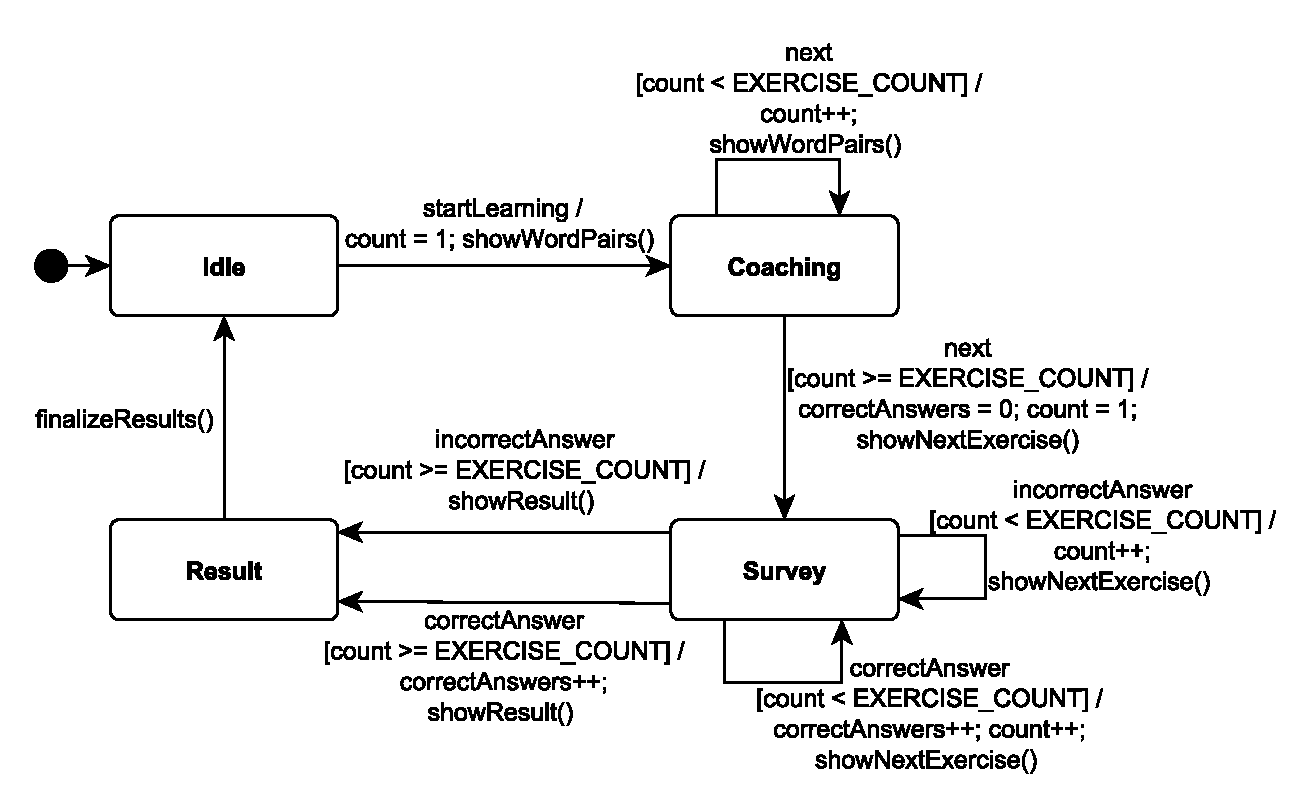
\includegraphics{figures/business-logic.pdf}
     	}
     	\caption{A leckék kezelését segítő ablak.}
     	\label{fig:business-logic}
     \end{figure}
 
 	A felhasználó bejelentkezése után az alkalmazás alapállapotba (\emph{Idle}) kerül, innen lehet elkezdeni egy lecke megtanulását (\emph{Start Learning!}~gomb). Az alkalmazás ekkor a tanító állapotba kerül (\emph{Coaching}), ahol bemutatja, hogy milyen szópárokat kell memorizálni. Ha az összes szópárt bemutatta, elkezdődik a kikérdező fázis (\emph{Survey}), ahol a felhasználónak a jó válaszokat kell adni a kérdésekre. A jó válaszokat az alkalmazás számolja. A lecke végén a felhasználó megtekintheti eredményeit (\emph{Result}). Ezután az alkalmazás elmenti az eredményeket és visszakerül alapállapotba.
     
     \textbf{Megjelenés a kódban:} \textit{language.learning.client} package-ben a \textit{Controller.java} osztály.
     
     \subsubsection{Szolgáltatás hozzáférési réteg: ServiceAccess osztály}
     
     A ServiceAccess osztály felelős a szerver elérésért. Megvalósítja \aref{sec:interfészek}.~fejezetben ismertetett interfészeket. Egy interfész megvalósítása abból áll, hogy létrehoz egy alkalmas RestEasy\footnote{http://resteasy.jboss.org/} kliens objektumot, amelynek megadja a szerver elérhetőségét, majd delegálja a kapott hívást a létrehozott objektumnak.
     
     \textbf{Megjelenés a kódban:} \textit{language.learning.client} package-ben a \textit{ServiceAccess.java} osztály.
     
    \section{Telepítési útmutató}
    \label{sec:telepítés}
    Az alkalmazás használatához a következő programok szükségesek:
    \begin{itemize}
    	\item Java 8,
    	\item Maven 3.3,
    	\item WildFly 10.1.
    \end{itemize}

	Az alkalmazás használatához először el kell indítani a szervert. Ehhez nyitni kell egy \emph{parancssort} és bele kell navigálni a szerver projektbe (\textsl{language.learning.server}). Itt ki kell adni a következő parancsokat:
\begin{lstlisting}[
basicstyle=\small, %or \small or \footnotesize etc.
]
mvn package
mvn wildfly:deploy
\end{lstlisting}
	A szerver ezek után elérhető lesz.
	
	A kliens elindításához csupán a \textsl{language.learning.client} fájlt kell elindítani, az elindulást a grafikus felület megjelenése mutatja.
	
	\section{Összefoglalás}
	\label{sec:összefoglalás}
	Munkánk során megterveztük, megvalósítottuk és dokumentáltuk a Szoftver architektúrák tárgyra készített szótanuló alkalmazást. Az alkalmazás segítségével angol szavakat és kifejezéseket lehet tanulni.
	
	Az elkészített alkalmazás egy kliens-szerver architektúrát használ. Az alkalmazás az adatokat egy szerveren egy Oracle
	adatbázisban tárolja. A felhasználók az alkalmazást egy kliens segítségével grafikus felületen keresztül érhetik el. A kliens és szerver kommunikációja REST hívásokkal történik. 
	
	Munkánk során alaposan megterveztük a rendszert. A terveket magas minőséggel implementáltuk; az összes követelmény, amelyet a követelményspecifikációban megfogalmaztunk (kötelező és opcionális), megvalósításra került. Az alkalmazást gondosan teszteltük, a hibákat javítottuk, így a program megbízhatónak és stabilnak mondható.
	
	Kiterjesztési lehetőségként a következő pontokat azonosítottuk:
	\begin{itemize}
		\item további feladattípusok felvétele,
		\item felhasználó által összeállítható leckék támogatása,
		\item kliensek készítése más platformokon (okostelefon, webes felület).
	\end{itemize}
\end{document}